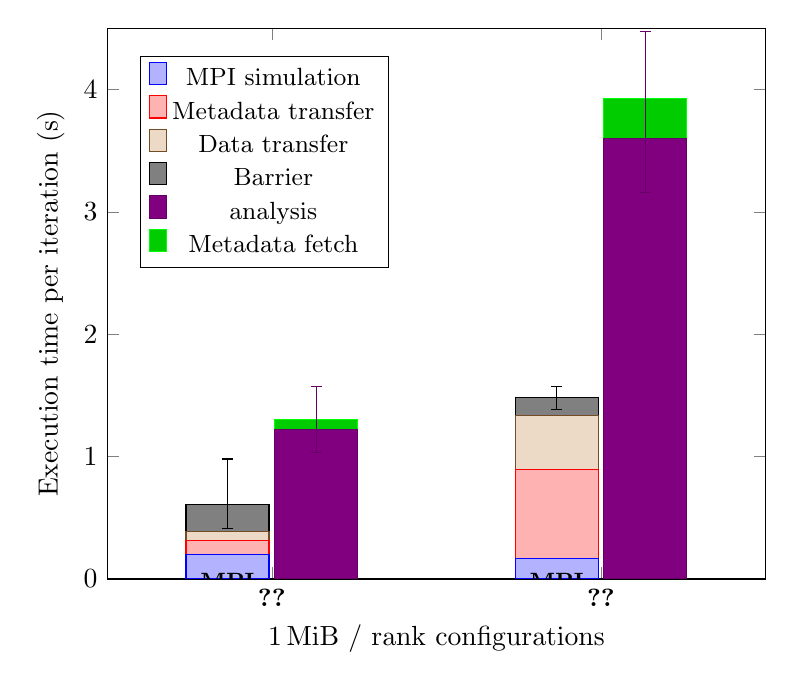
\begin{tikzpicture}[
/pgfplots/every axis/.style={ % <- added /pgfplots/ 
    ybar stacked,
    ymin=0,
    ymax=4.5,
    ytick={0, 1, 2, 3, 4},
    symbolic x coords={411, 1641},
    bar width=30pt,
    legend style={font=\small, at={(0.05,0.95)},anchor=north west},
    ylabel={Execution time per iteration (s)},
    xlabel={1\,MiB / rank configurations},
    xtick=data,
    xticklabels={\ref{XP2.1.128},\ref{XP2.1.512}},
    x tick label style={font=\small,},
    hide axis,
    width=.82\columnwidth,
    enlarge x limits={rel=0.5},
    point meta=explicit symbolic,
  }, 
]
\begin{axis}[bar shift=-16pt, hide axis=false]
\legend{MPI simulation, Metadata transfer, Data transfer, Barrier, \dask analysis, Metadata fetch}
\addplot coordinates { (411,0) (1641,0) };
\addplot coordinates { (411,0) (1641,0) };
\addplot coordinates { (411,0) (1641,0) };
\addplot coordinates { (411,0) (1641,0) };
\addplot coordinates { (411,0) (1641,0) };
\addplot coordinates { (411,0) (1641,0) };
\end{axis}

%%%%%%%%%%%%%% 1M %%%%%%%%%%%%%%%%%%%%%%%%%%%%%%%%%%%%%%%%%%%%%%%%%

%meansimu =   [0.20378826092928648,  0.16849265048716688]
%meandask =  [1.2227224971564417, 3.60005530453701]
%meanputq= [0.11280882632812943,  0.7232108102396827]
%meangetq= [0.08205931478490432,  0.32900929676058394]
%meanscatter= [0.07447400204512178,  0.4456939545007496]
%meanbar= [0.21443583569608413,  0.1472610141856876]

%iter =  [Max( MPI:0.6073631280990716, Dask: 1.304781811941346 ),Max ( MPI: 1.486193363804432, Dask : 3.929064601297594 )]
% 2%*iter = [0.02609563623882692, 0.07858129202595188]

%%%%%%%%%%%%%%%%%%%%%%%%%%%%%%%%%%%%%%%%%%%%%%%%%%%%%%%%%%%%%%%%%%%%%%%%%%%

%%%% MPI %%%%
\begin{axis}[xshift=-16pt]
\node[coordinate,pin={{\footnotesize\bfseries MPI}}] at (411,-.45) {};
\node[coordinate,pin={{\footnotesize\bfseries MPI}}] at (1641,-.45) {};

%stdsimu =  [0.028907557788677447,  0.00656858080088586] : [0.02609563623882692, 0.07858129202595188]
%Min simu =  [0.17287868517973948,  0.16206971241592782]
%Mean simu =  [0.20378826092928648,  0.16849265048716688] 
%Max simu [0.23015613693451087,  0.17519777858422003]


\addplot+[error bars/.cd, y dir=both, y explicit]  %simu
         coordinates { (411,0.203)
                       %+- (,0.00656858080088586) % < 0.02609563623882692
                       (1641,0.168)
                       % +- (,0.00656858080088586) % < 0,0.02972386727
                     };
%stdputq =  [0.005781409824694809,  0.009123255592682601] : < [0.02609563623882692, 0.07858129202595188]
%Min putq =  [0.10689240859187521,  0.7171006665419668]
%Mean putq =  [0.11280882632812943,  0.7232108102396827]
%Max putq [0.11844503826546315,  0.733697799782135]


\addplot+[error bars/.cd, y dir=both, y explicit]  %putq
         coordinates { (411,0.11280882632812943)
                       % +- (,0.005781409824694809) % < 0.02609563623882692
                       (1641,0.7232108102396827)
                       % +- (,0.009123255592682601) % < 0.07858129202595188
                      };
%stdscatter =  [0.022278990461730694, 0.06619416442538288] : < [0.02609563623882692, 0.07858129202595188]
%Min scatter =  [0.05815409594345056,  0.4070897154490467]
%Mean meanscatter =  [0.07447400204512178,  0.4456939545007496]
%Max scatter [0.0998560024370363,  0.5221270809265661]


\addplot+[error bars/.cd, y dir=both, y explicit]  %scatter
         coordinates { (411,0.07447400204512178)
                       %+- (,0.022278990461730694)
                       (1641,0.4456939545007496)
                       %+- (,0.06619416442538288)
                      };
%stdbar =  [0.3250447445341635,  0.09527162041058722] : > [0.02609563623882692, 0.07858129202595188]
%Min bar =  [0.024776848883675484, 0.046745352296341025]
%Mean bar =  [0.21443583569608413,  0.1472610141856876]
%Max bar [0.5897580874584492,  0.23623748330203398]

\addplot+[error bars/.cd, y dir=both, y explicit]  %bar
         coordinates { (411,0.21443583569608413)
                       += (,0.375322251762365) -= (,0.18965898681240864)
                       (1641,0.1472610141856876)
                       += (,0.08897646911634638) -= (,0.10051566188934657)
                      };
\addplot coordinates { (411,0)     (1641,0)     }; %dask
\addplot coordinates { (411,0)     (1641,0)     }; %getq
\end{axis}

%%%% Dask %%%%
\begin{axis}[xshift=16pt] 
\node[coordinate,pin={{\footnotesize\bfseries \dask}}] at (411,-.45) {};
\node[coordinate,pin={{\footnotesize\bfseries \dask}}] at (1641,-.45) {};
\addplot coordinates { (411,0)     (1641,0)     }; %simu
\addplot coordinates { (411,0)     (1641,0)     }; %putq
\addplot coordinates { (411,0)     (1641,0)     }; %scatter
\addplot coordinates { (411,0)     (1641,0)     }; %bar
%stddask =  [0.3015011760477324, 0.7588320784454731] : > [0.02609563623882692, 0.07858129202595188]
%Min dask =  [1.0339068029231082, 3.157302851245428]
%Mean dask =  [1.2227224971564417, 3.60005530453701]
%Max dask [1.5704373405573682, 4.476262671329702]


\addplot+[error bars/.cd, y dir=both, y explicit]  %dask
         coordinates { (411,1.2227224971564417)
                       += (,0.3477148434009265) -= (,0.18881569423333344)
                       (1641,3.60005530453701)
                       += (,0.8762073667926922) -= (,0.4427524532915821)
                      };
%stdgetq =  [0.0015614752884921415, 0.012205066604482485] : < [0.02609563623882692, 0.07858129202595188]
%Min getq =  [0.08025651518255472,  0.3181074700421757]
%Mean getq =  [0.08205931478490432,  0.32900929676058394]
%Max getq [0.0829860181806402,  0.3421949552009917]


\addplot+[error bars/.cd, y dir=both, y explicit]  %getq
         coordinates { (411,0.08205931478490432)
                       % +- (,0.0015614752884921415) % < 0,00807149734339
                       (1641,0.32900929676058394)
                       % +- (,0.012205066604482485) % < 0,0263540142663
                      };
\end{axis}

\end{tikzpicture}



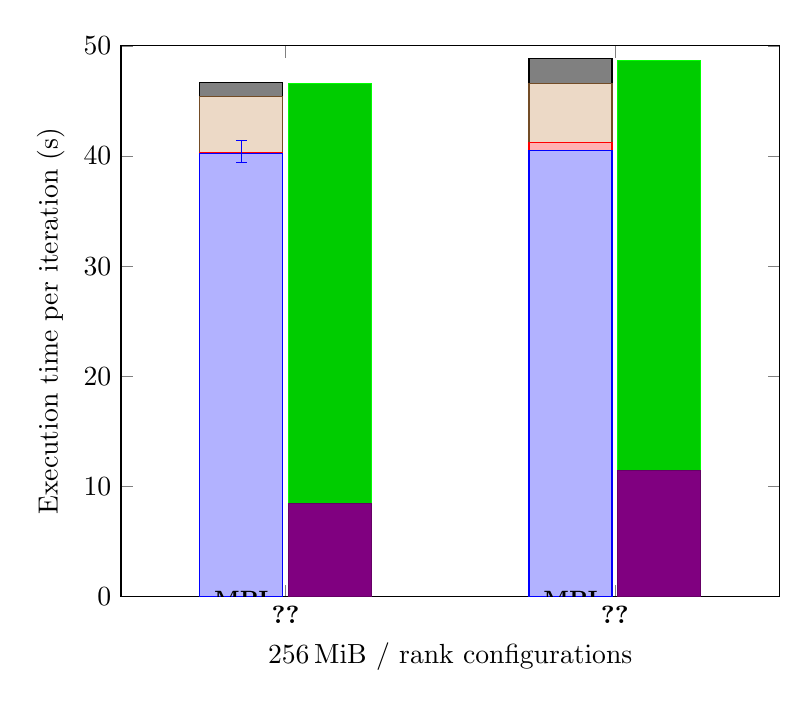
\begin{tikzpicture}[
/pgfplots/every axis/.style={ % <- added /pgfplots/ 
    ybar stacked,
    ymin=0,
    ymax=50,
    ytick={0, 10, 20, 30, 40, 50},
    symbolic x coords={ 41256, 164256},
    bar width=30pt,
    %legend style={font=\small, at={(0.05,0.9)},anchor=south east},
    ylabel={Execution time per iteration (s)},
    xlabel={256\,MiB / rank configurations},
    xtick=data,
    xticklabels={\ref{XP2.256.128},\ref{XP2.256.512}},
    x tick label style={font=\small,},
    hide axis,
    width=.82\columnwidth,
    enlarge x limits=0.5,
    point meta=explicit symbolic,
  },
]
\begin{axis}[bar shift=-16pt, hide axis=false]
\addplot coordinates { (41256,0) (164256,0) };
\addplot coordinates { (41256,0) (164256,0) };
\addplot coordinates { (41256,0) (164256,0) };
\addplot coordinates { (41256,0) (164256,0) };
\addplot coordinates { (41256,0) (164256,0) };
\addplot coordinates { (41256,0) (164256,0) };
\end{axis}

%%%%%%%%%%%%%%%%%% 256M %%%%%%%%%%%%%%%%%%%%%%%%%%%%%%%%%%%%%%%%

%meansimu =  [40.19396744045631, , 40.474843232321064]
%meandask =  [8.410617398468917,  11.448131603119826]
%meanputq= [0.0795850563008192,  0.7631853370359067]
%meangetq= [38.19960798663777, 37.22121849190444]
%meanscatter= [5.147044166001099,  5.316233275613153]
%meanbar= [1.253565882761298,  2.259944601142744]


%MPI iter =  [46.67603649275399,  48.81615962772145]
%Dask  = [46.61022538510669, 48.669350095024264]
%iter =  [Max( MPI, Dask: ),Max ( MPI: , Dask :  )] = 
%iter = MPI iter = [46.67603649275399,  48.81615962772145]
% 2%*iter = [0.9322045077021338, 0.9733870019004853]

%%%%%%%%%%%%%%%%%%%%%%%%%%%%%%%%%%%%%%%%%%%%%%%%%%%%%%%%%%%%

%%%% MPI %%%%
\begin{axis}[xshift=-16pt]
\node[coordinate,pin={{\footnotesize\bfseries MPI}}] at (41256,-5) {};
\node[coordinate,pin={{\footnotesize\bfseries MPI}}] at (164256,-5) {};
%stdsimu =  [1.0833717427874794,  0.4051487721548612] : [>0.9322045077021338, <0.9733870019004853]
%Min simu =  [39.44312698278668,  40.13795151070883]
%Mean simu =  [40.19396744045631, 40.474843232321064]
%Max simu [41.43591711969384,  40.924400287337676]

\addplot+[error bars/.cd, y dir=both, y explicit]  %simu
         coordinates { (41256,40.19396744045631)
                       += (,1.2419496792375284) -= (,0.7508404576696321)
                       (164256,40.474843232321064) 
                       %+- (,0.4051487721548612) % < 0.976323192554
                      };
%stdputq =  [0.007874413545552569, 0.07190917364509905]< [0.9322045077021338, 0.9733870019004853]
%Min putq =  [0.07086614267359437, 0.6901729620151968]
%Mean putq =  [0.0795850563008192,  0.7631853370359067]
%Max putq [0.08617874621711508,  0.8339380437080308]

\addplot+[error bars/.cd, y dir=both, y explicit]  %putq
         coordinates { (41256,0.0795850563008192)
                       % +- (,0.007874413545552569) % < 0.933520729855
                       (164256,0.7631853370359067) 
                       %+- (,0.07190917364509905) % < 0.976323192554
                      };
%stdscatter =  [0.22428716130564308,  0.24283345436052847] <[0.9322045077021338, 0.9733870019004853]
%Min scatter =  [4.8977906801026165,  5.168739588378514
%Mean meanscatter =  [5.147044166001099,5.316233275613153]
%Max scatter [5.332574566903986,  5.5965044415901275]

\addplot+[error bars/.cd, y dir=both, y explicit]  %scatter
         coordinates { (41256,5.147044166001099)
                       % +- (,0.22428716130564308) % < 0.933520729855
                       (164256,5.316233275613153)
                       % +- (,0.24283345436052847) % < 0.976323192554
                       };
%stdbar =  [0.0890767570792701,  0.6896973362478515] < [0.9322045077021338, 0.9733870019004853]
%Min bar =  [1.1664388556512222, 1.747406680871677]
%Mean bar =  [1.253565882761298,  2.259944601142744]
%Max bar [1.3444720780314583,  3.044097142989756]
\addplot+[error bars/.cd, y dir=both, y explicit]  %bar
         coordinates { (41256,1.253565882761298)
                       % +- (,0.0890767570792701) % < 0.933520729855
                       (164256,2.259944601142744)
                       % +- (,0.6896973362478515) % < 0.976323192554
                       };
\addplot coordinates { (41256,0)     (164256,0)     }; %dask
\addplot coordinates { (41256,0)     (164256,0)     }; %getq
\end{axis}

%%%% Dask %%%%
\begin{axis}[xshift=16pt] 
\node[coordinate,pin={{\footnotesize\bfseries \dask}}] at (41256,-5) {};
\node[coordinate,pin={{\footnotesize\bfseries \dask}}] at (164256,-5) {};
\addplot coordinates { (41256,0)     (164256,0)     }; %simu
\addplot coordinates { (41256,0)     (164256,0)     }; %putq
\addplot coordinates { (41256,0)     (164256,0)     }; %scatter
\addplot coordinates { (41256,0)     (164256,0)     }; %bar
%stddask =  [0.11870514435554211,  0.5837459627450405] < [0.9322045077021338, 0.9733870019004853]
%Min dask =  [8.329631023703971, 10.896099947574031]
%Mean dask =  [8.410617398468917, 11.448131603119826]
%Max dask [8.54688018762196,  12.059117784025148]

\addplot+[error bars/.cd, y dir=both, y explicit]  %dask
         coordinates { (41256,8.410617398468917)
                       % +- (,0.11870514435554211) % < 0.933520729855
                       (164256,11.448131603119826)
                       % +- (,0.5837459627450405) % < 0.976323192554
                       };
%stdgetq =  [0.8944936599264665,  0.05439716415244653] < [0.9322045077021338, 0.9733870019004853]
%Min getq =  [37.65883787051361,  37.182585414266214]
%Mean getq =  [38.19960798663777,  37.22121849190444]
%Max getq [39.23209190231541,  37.28342635212984]

\addplot+[error bars/.cd, y dir=both, y explicit]  %getq
         coordinates { (41256,38.19960798663777)
                       % +- (,0.8944936599264665) % < 0.933520729855
                       (164256,37.22121849190444)
                       % +- (,0.05439716415244653) % < 0.976323192554
                       };
\end{axis}

\end{tikzpicture} 

